
\appendix
%\appendixpage
%\addappheadtotoc
\chapter{Testübersicht}
\label{app:Testfälle}
Die folgenden Informationen sollen eine Übersicht über die Funktionalitäten zu geben, welche im  \cref{app:Funktionalitäten} \nameref{app:Funktionalitäten} beschrieben werden.

Der Abschnitt \textit{Ablauf} zeigt den Zustandsgraphen auf, welcher bei den Tests eingehalten werden muss. \textit{Test Cases} zeigt die verschiedenen Eingabeparameter, welche benötigt werden, um die gesamte Funktionalität testen zu könnenn. Die \textit{Top 10 Destinationen} werden benötigt, um die Smoke Tests zu entwickeln (siehe \cref{sec:konzept:smoketests} \nameref{sec:konzept:smoketests}).

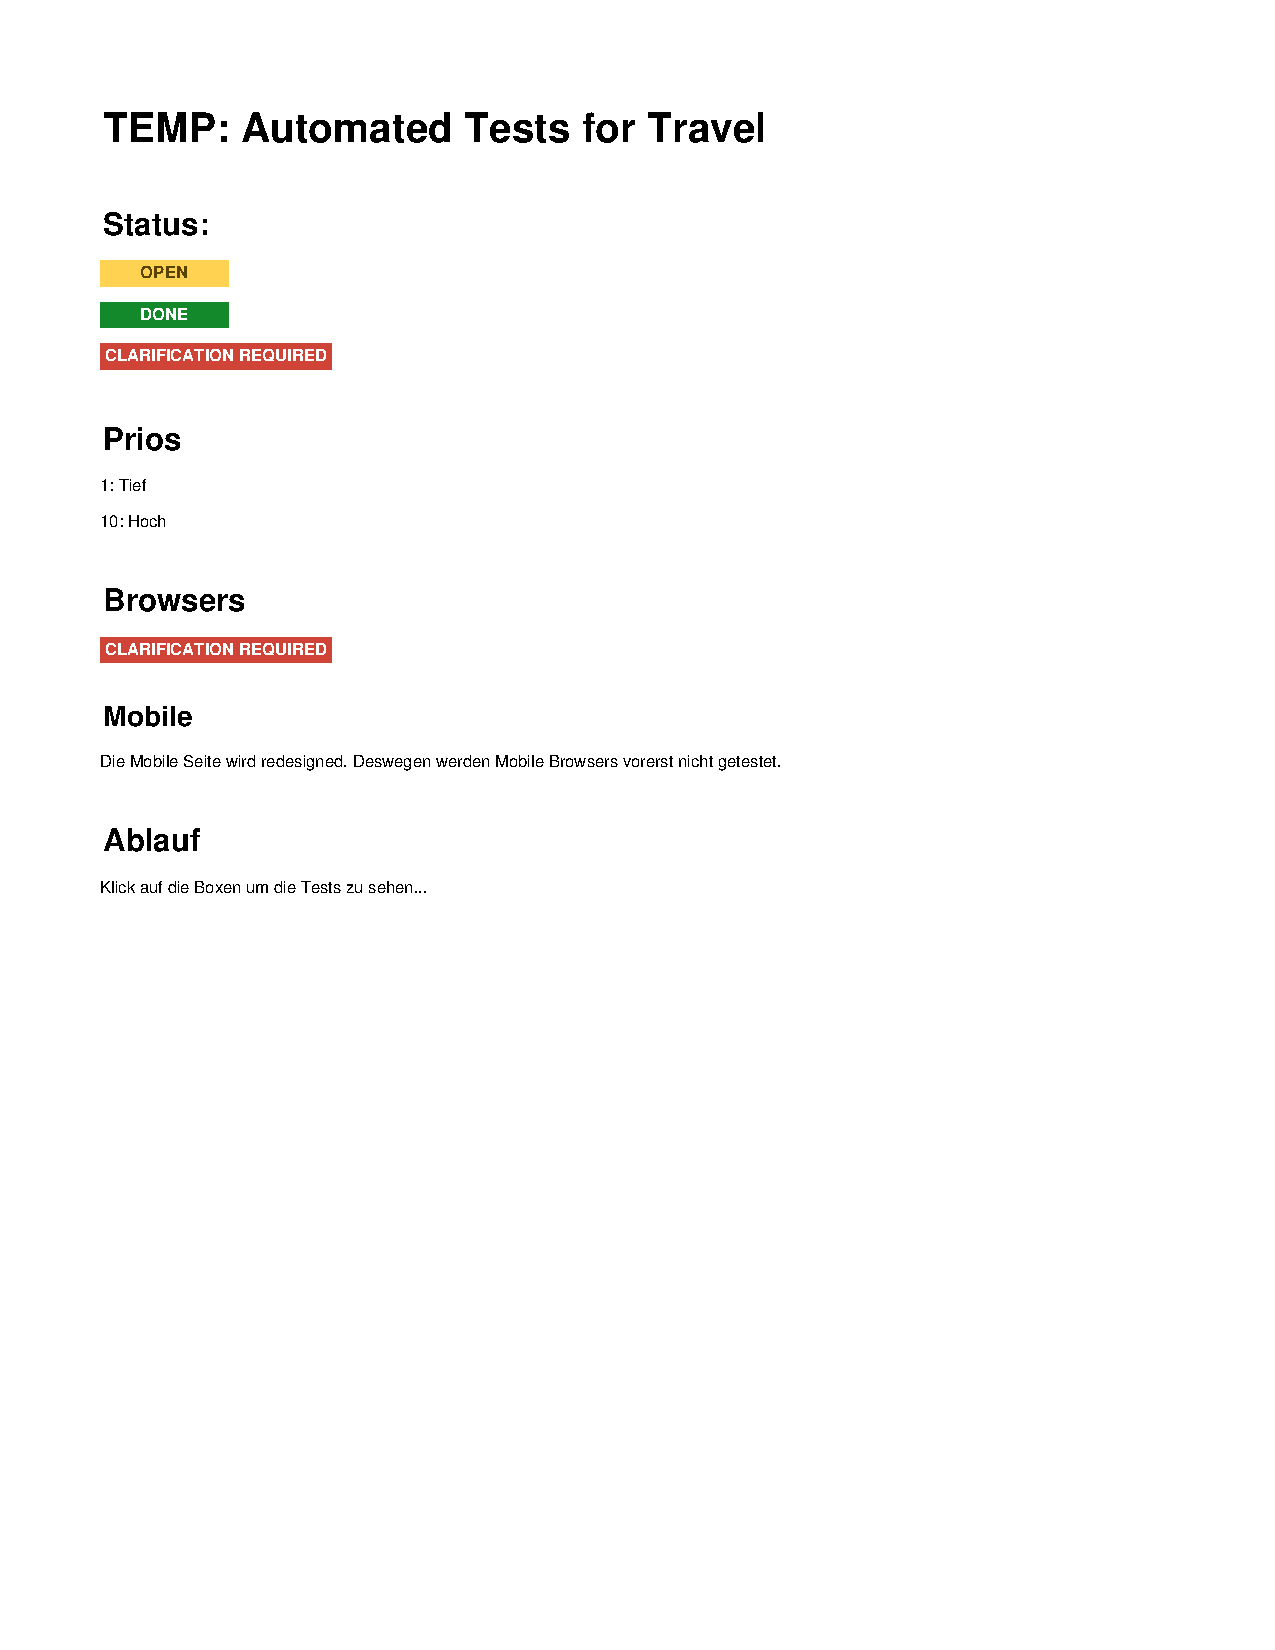
\includepdf[scale=0.8,pages=1,pagecommand=\section{Testübersicht}]{./../test-documentation-1-overview.pdf}
\includepdf[scale=0.8,pages=2,pagecommand=\subsubsection{}]{./../test-documentation-1-overview.pdf}
\includepdf[scale=0.8,pages=3,pagecommand=\subsubsection{}]{./../test-documentation-1-overview.pdf}
\includepdf[scale=0.8,pages=4,pagecommand=\subsubsection{}]{./../test-documentation-1-overview.pdf}
\includepdf[scale=0.8,pages=5,pagecommand=\subsubsection{}]{./../test-documentation-1-overview.pdf}

\chapter{Funktionalitäten}
\label{app:Funktionalitäten}
Folgend ist die gesamte Funktionalität der Travel.ch Webseite aufgeführt. Aufgeteilt sind die Funktionalität nach den Webseiten, auf welchen sie angezeigt werden.

Die wichtigsten Felder ist die \textit{Beschreibung}, der \textit{Status} und die \textit{Priorität}. Die Beschreibung erläutert die Funktionalität. Der Status zeigt an, ob eine Funktionalität noch zu testen ist (OPEN), bereits getestet ist (DONE), oder weitere Abklärungen benötigt werden (CLARIFICATION REQUIRED). Die Prioritäten sind in einer Skala von 1 bis 10 angegeben, wobei 10 am dringlichsten ist und 1 am unwichtigsten.

Zur Einteilung der Funktionalitäten sind die beiden Felder \textit{Kategorie} und \textit{Engine} vorhanden. Die Spalte "`Notizen"' mit einer Frage befüllt werden, wenn der Status auf CLARIFICATION REQUIRED gesetzt ist, oder sonstige Informationen beinhalten. \textit{Implemented in} soll den Entwicklern helfen die Übersicht zu behalten, welche Tests welche Funktionalitäten abdecken.


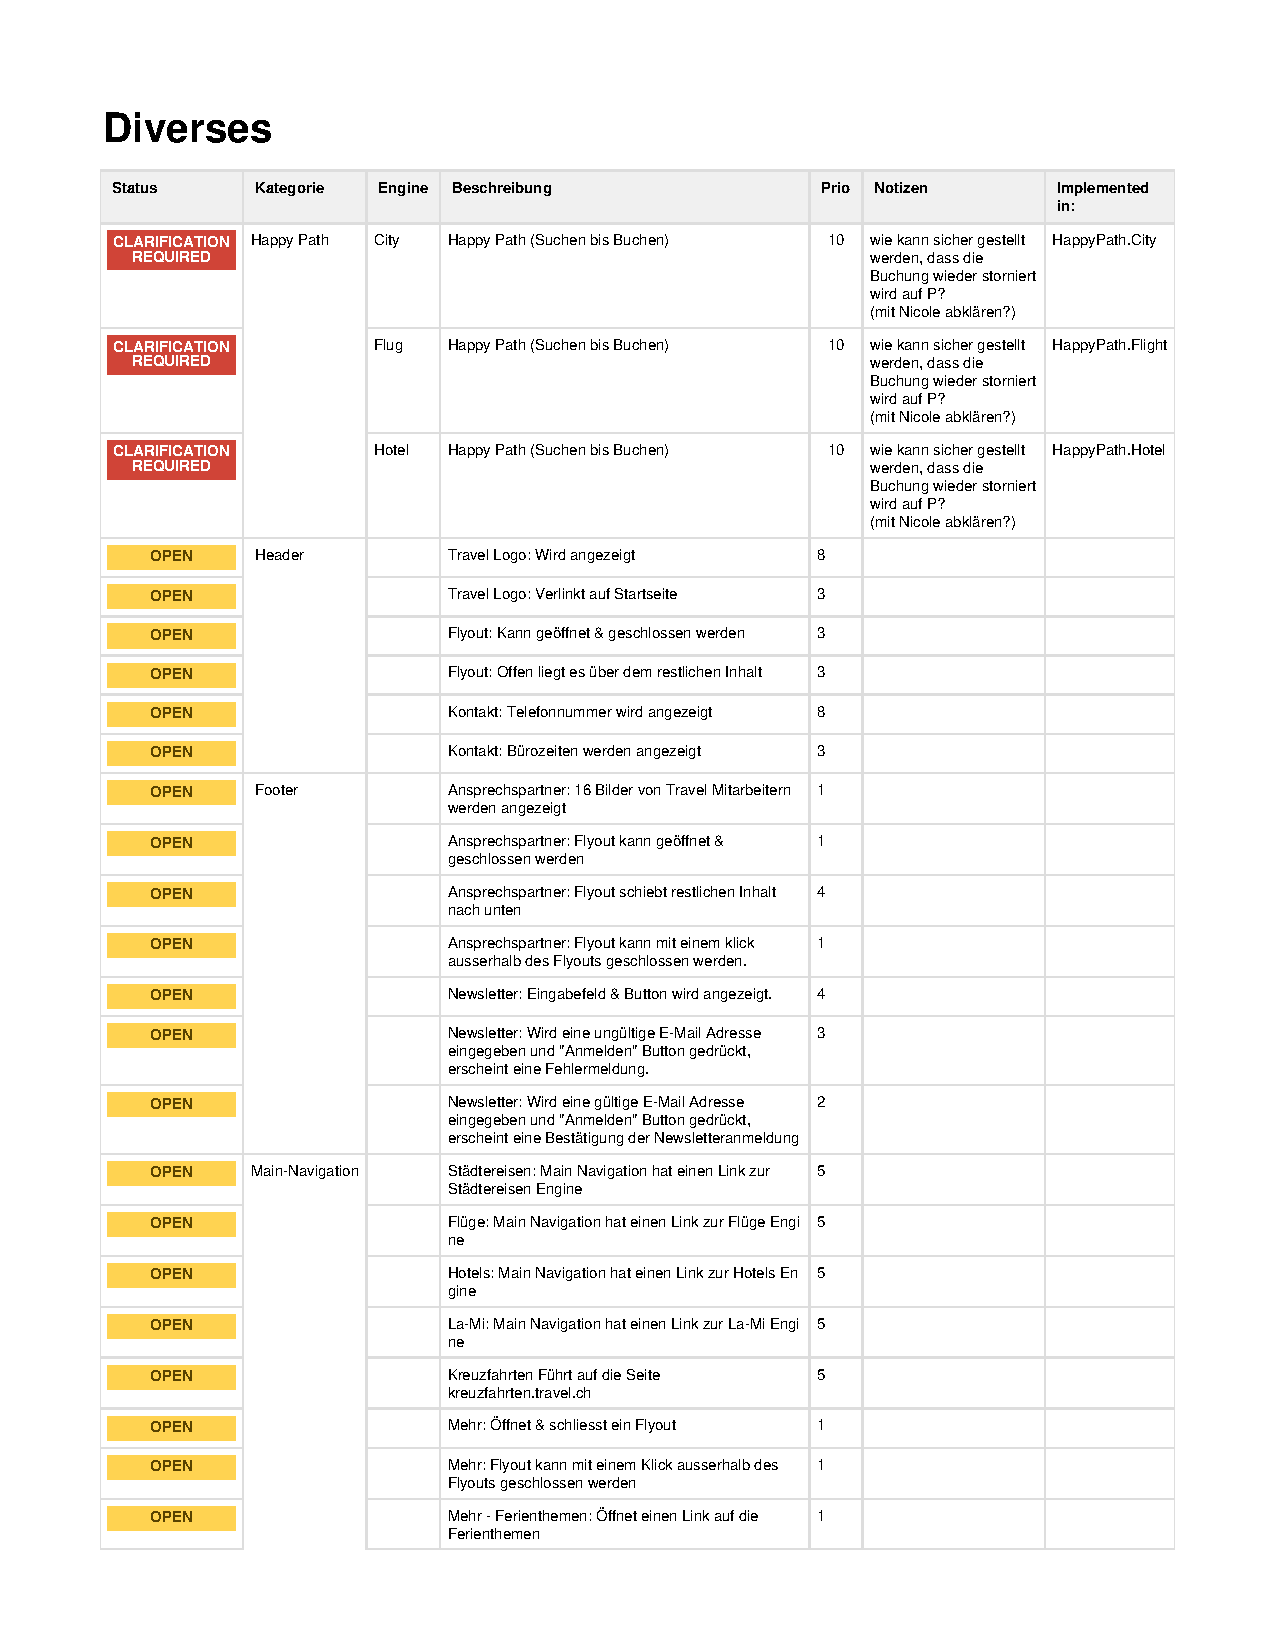
\includepdf[scale=0.8,pages=1,pagecommand=\section{Diverses}]{./../test-documentation-2-miscellaneous.pdf}
\includepdf[scale=0.8,pages=2,pagecommand=\subsubsection{}]{./../test-documentation-2-miscellaneous.pdf}


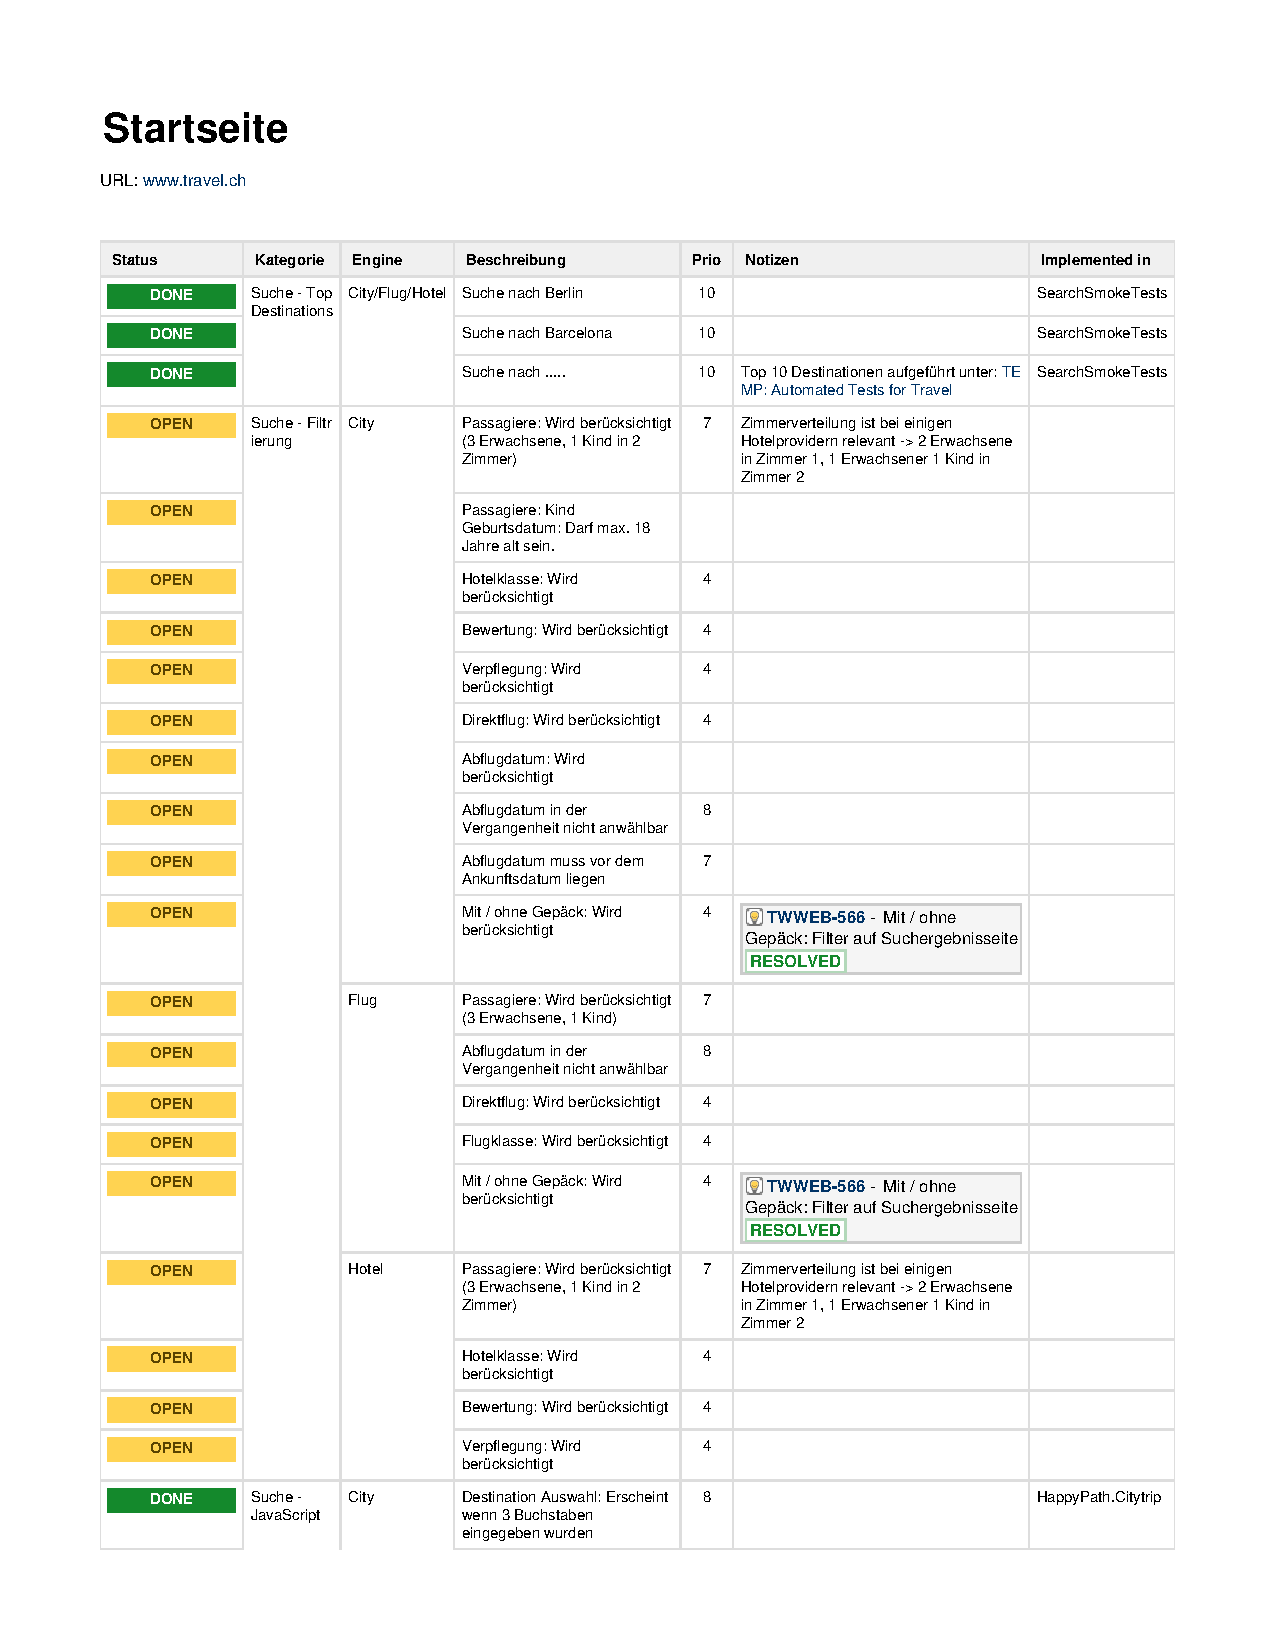
\includepdf[scale=0.8,pages=1,pagecommand=\section{Startseite}]{./../test-documentation-3-startpage.pdf}
\includepdf[scale=0.8,pages=2,pagecommand=\subsubsection{}]{./../test-documentation-3-startpage.pdf}
\includepdf[scale=0.8,pages=3,pagecommand=\subsubsection{}]{./../test-documentation-3-startpage.pdf}
\includepdf[scale=0.8,pages=4,pagecommand=\subsubsection{}]{./../test-documentation-3-startpage.pdf}


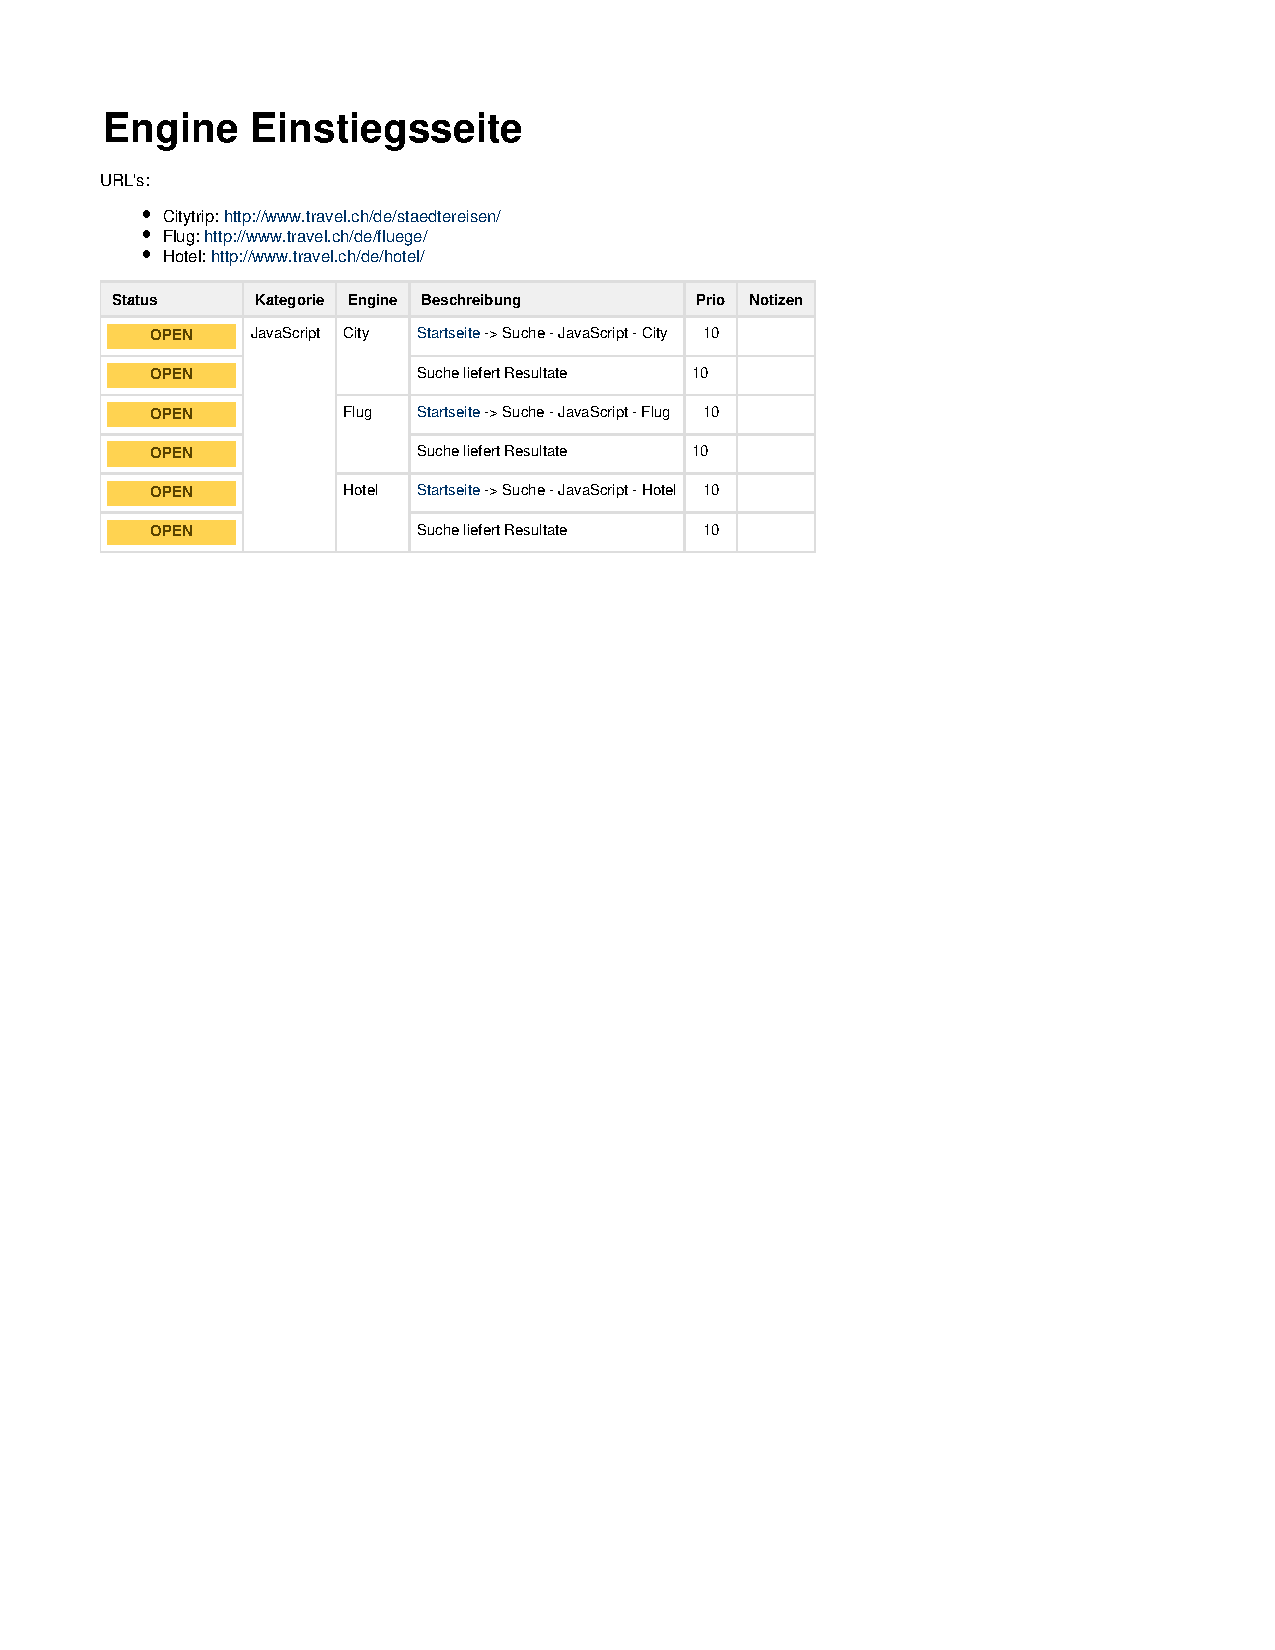
\includepdf[scale=0.8,pages=-,pagecommand=\section{Engine Startseite}]{./../test-documentation-4-engine-startpage.pdf}


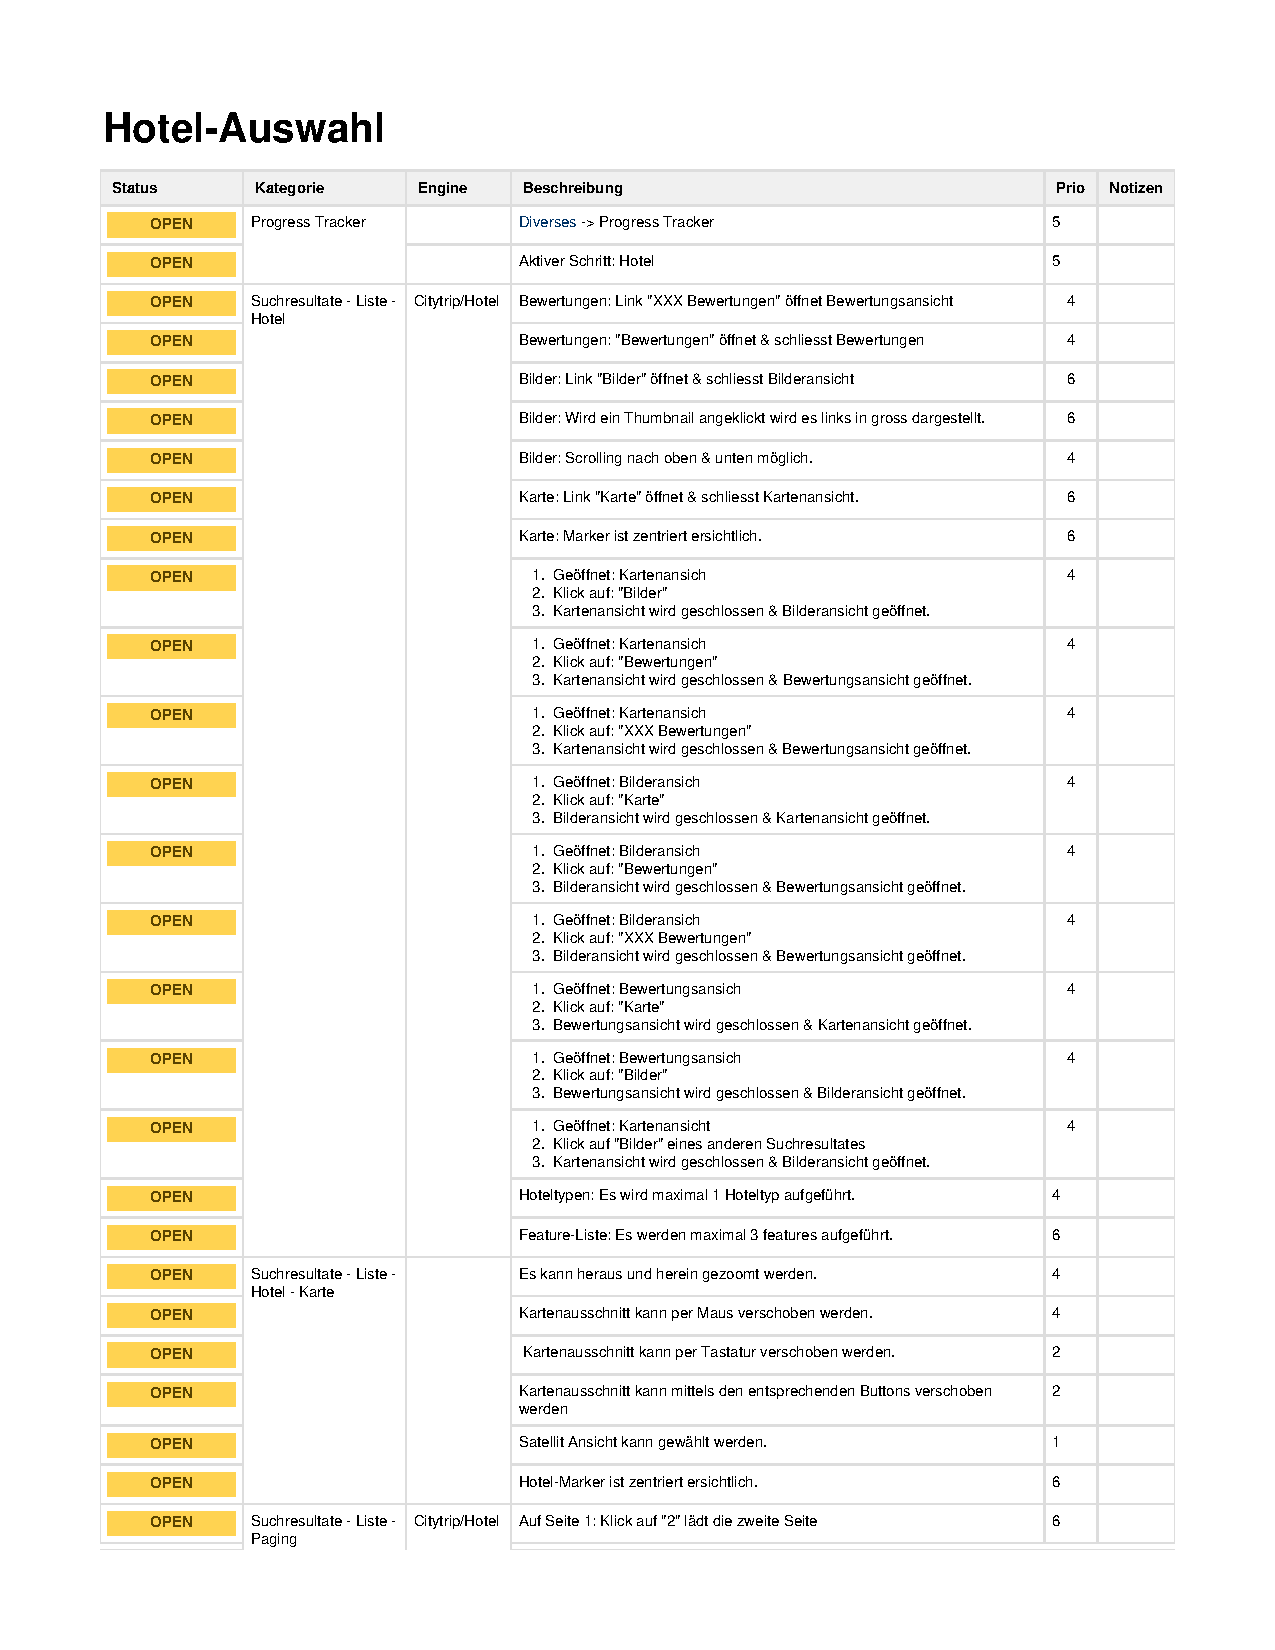
\includepdf[scale=0.8,pages=1,pagecommand=\section{Hotelauswahl}]{./../test-documentation-5-hotel-selection.pdf}
\includepdf[scale=0.8,pages=2,pagecommand=\subsubsection{}]{./../test-documentation-5-hotel-selection.pdf}
\includepdf[scale=0.8,pages=3,pagecommand=\subsubsection{}]{./../test-documentation-5-hotel-selection.pdf}


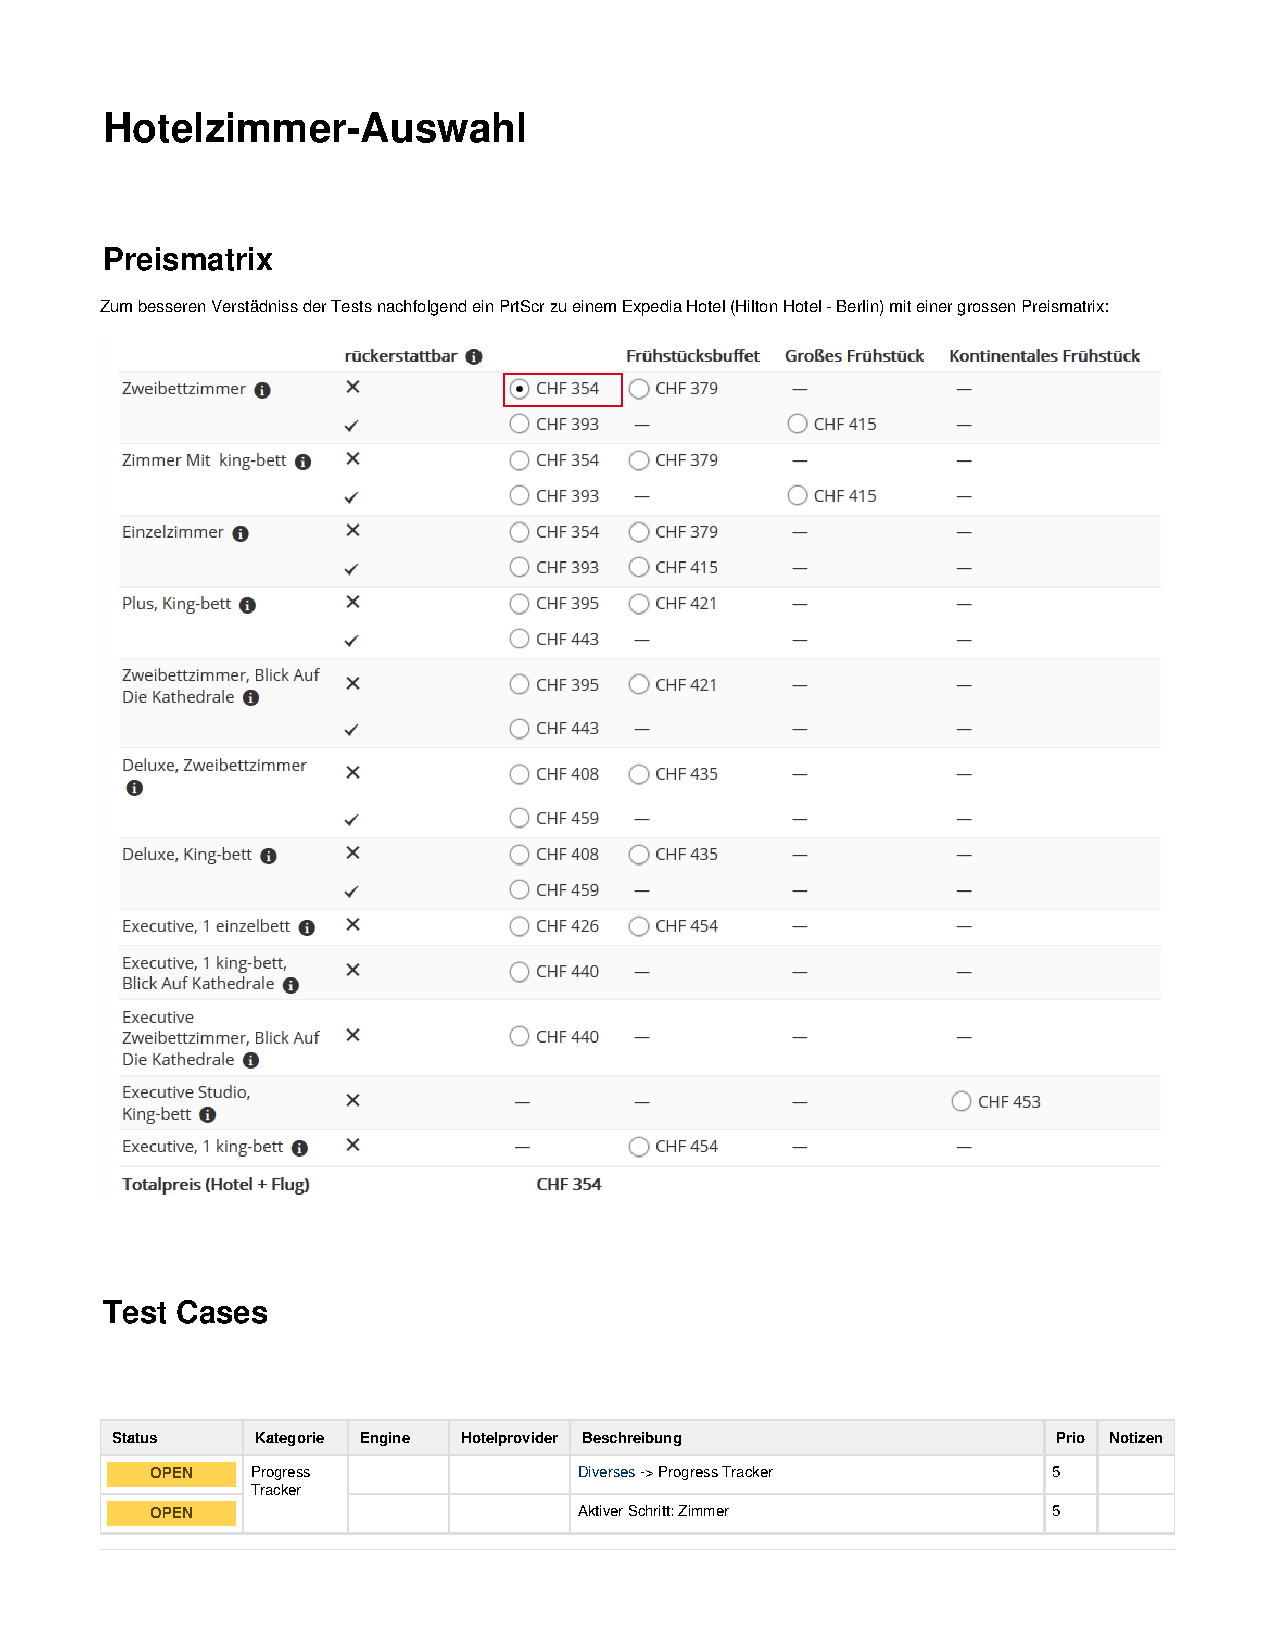
\includepdf[scale=0.8,pages=1,pagecommand=\section{Hotelzimmer Auswahl}]{./../test-documentation-6-hotelroom-selection.pdf}
\includepdf[scale=0.8,pages=2,pagecommand=\subsubsection{}]{./../test-documentation-6-hotelroom-selection.pdf}
\includepdf[scale=0.8,pages=3,pagecommand=\subsubsection{}]{./../test-documentation-6-hotelroom-selection.pdf}


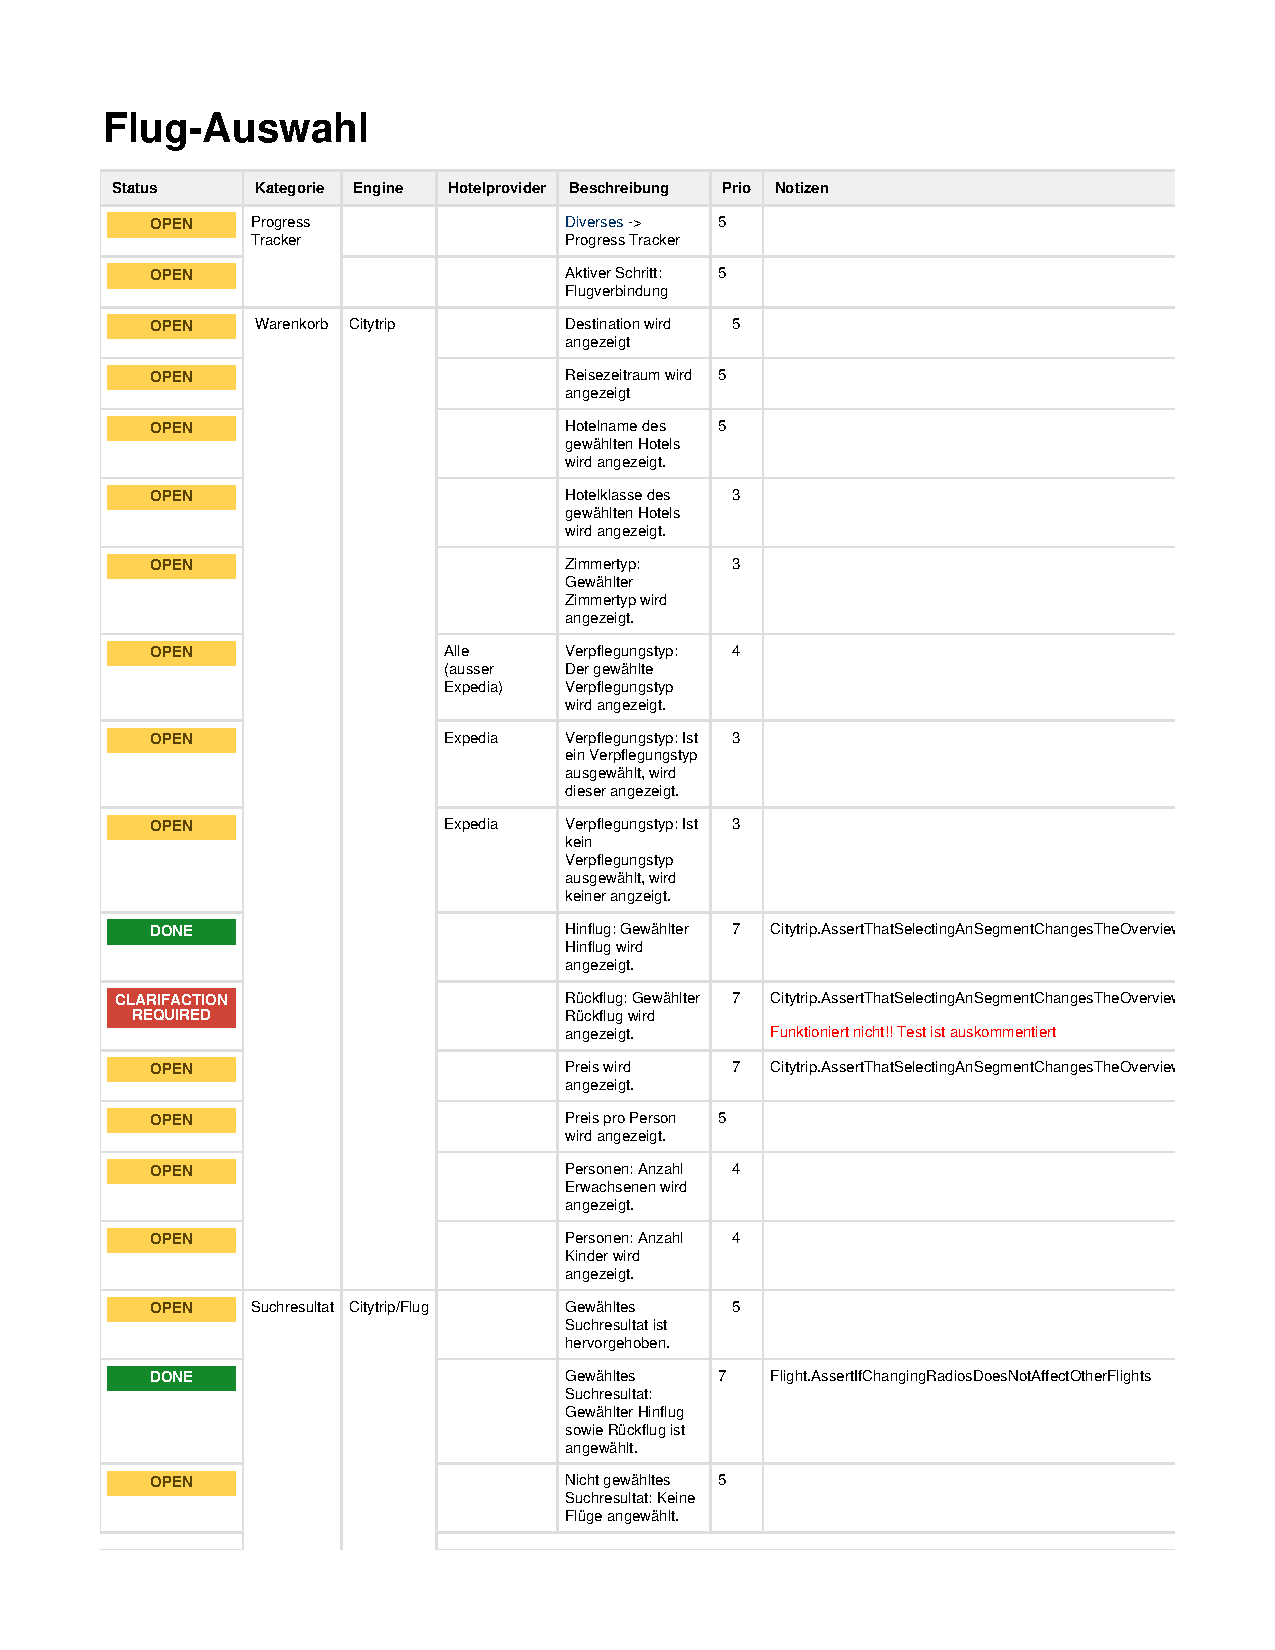
\includepdf[scale=0.8,pages=1,pagecommand=\section{Flugauswahl}]{./../test-documentation-7-flight-selection.pdf}
\includepdf[scale=0.8,pages=2,pagecommand=\subsubsection{}]{./../test-documentation-7-flight-selection.pdf}
\includepdf[scale=0.8,pages=3,pagecommand=\subsubsection{}]{./../test-documentation-7-flight-selection.pdf}


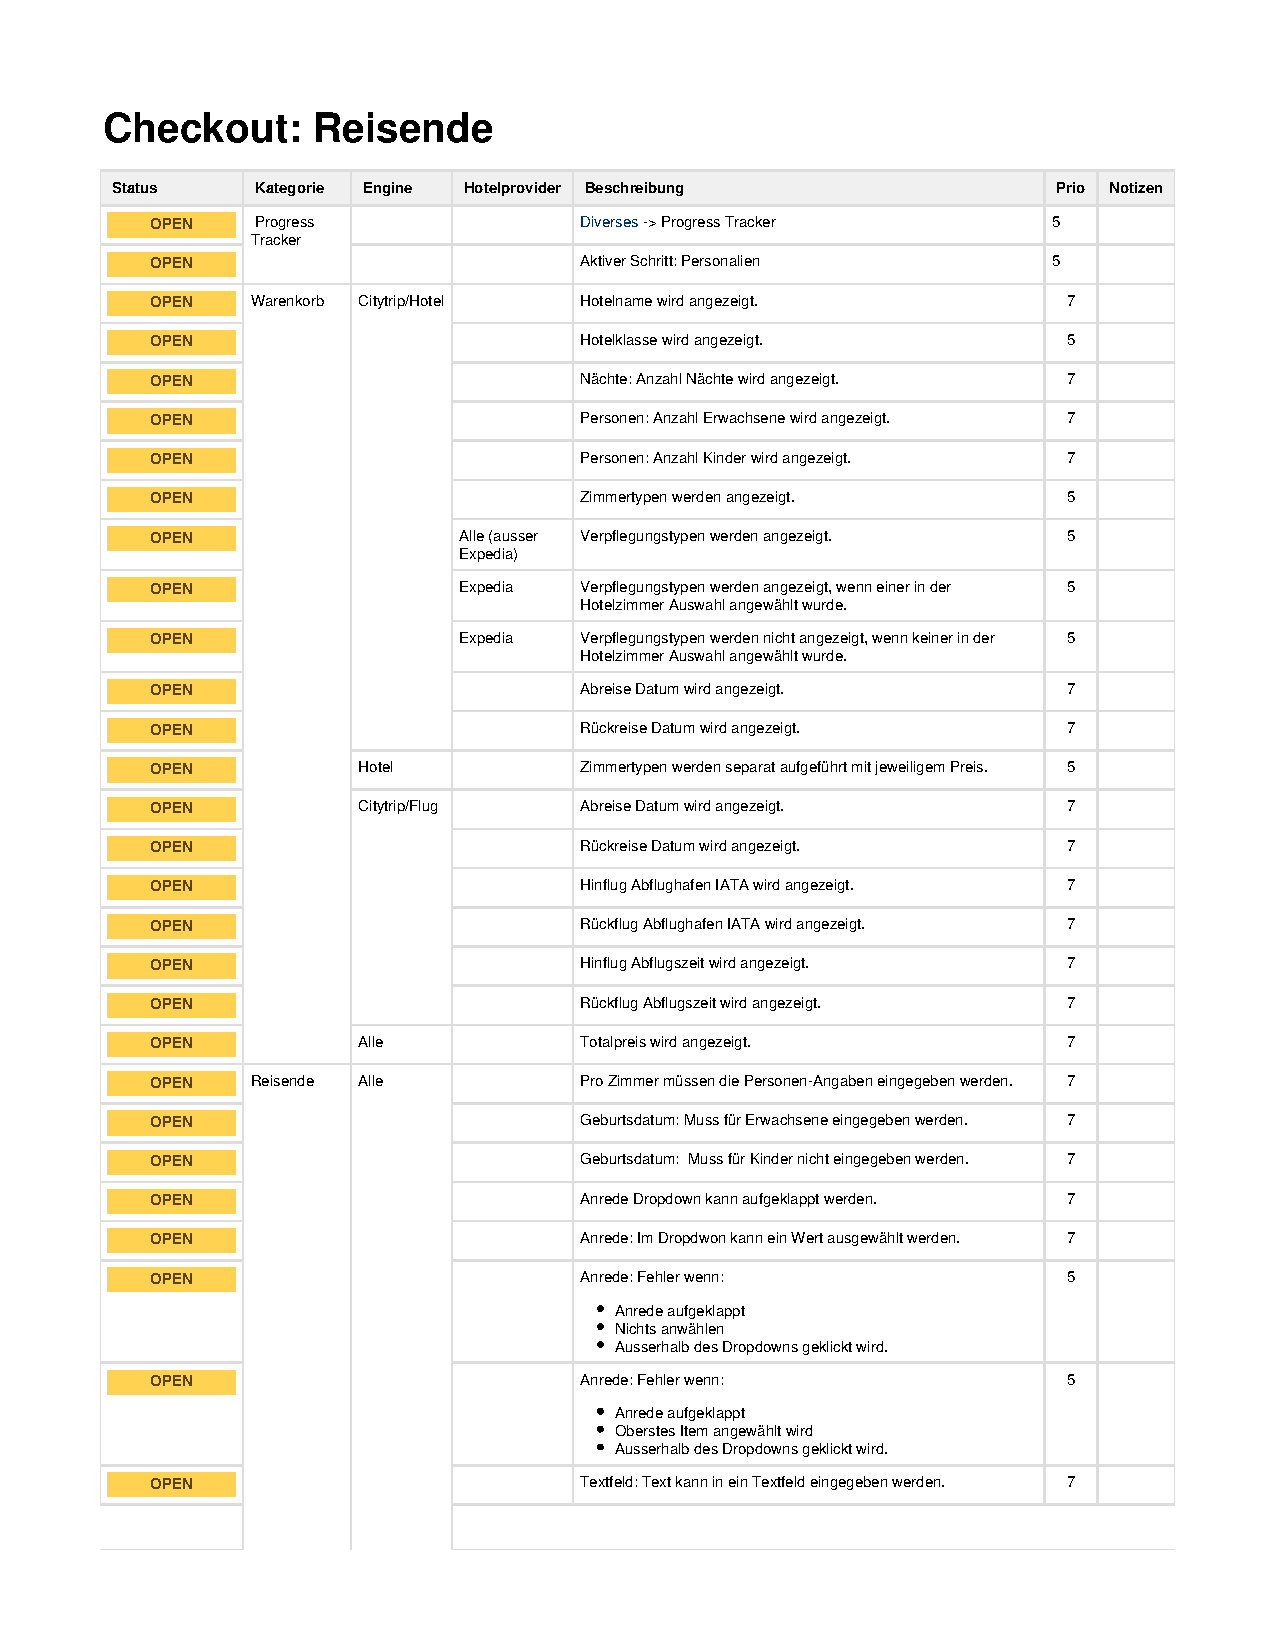
\includepdf[scale=0.8,pages=1,pagecommand=\section{Checkout: Passagiere}]{./../test-documentation-8-checkout-passengers.pdf}
\includepdf[scale=0.8,pages=2,pagecommand=\subsubsection{}]{./../test-documentation-8-checkout-passengers.pdf}


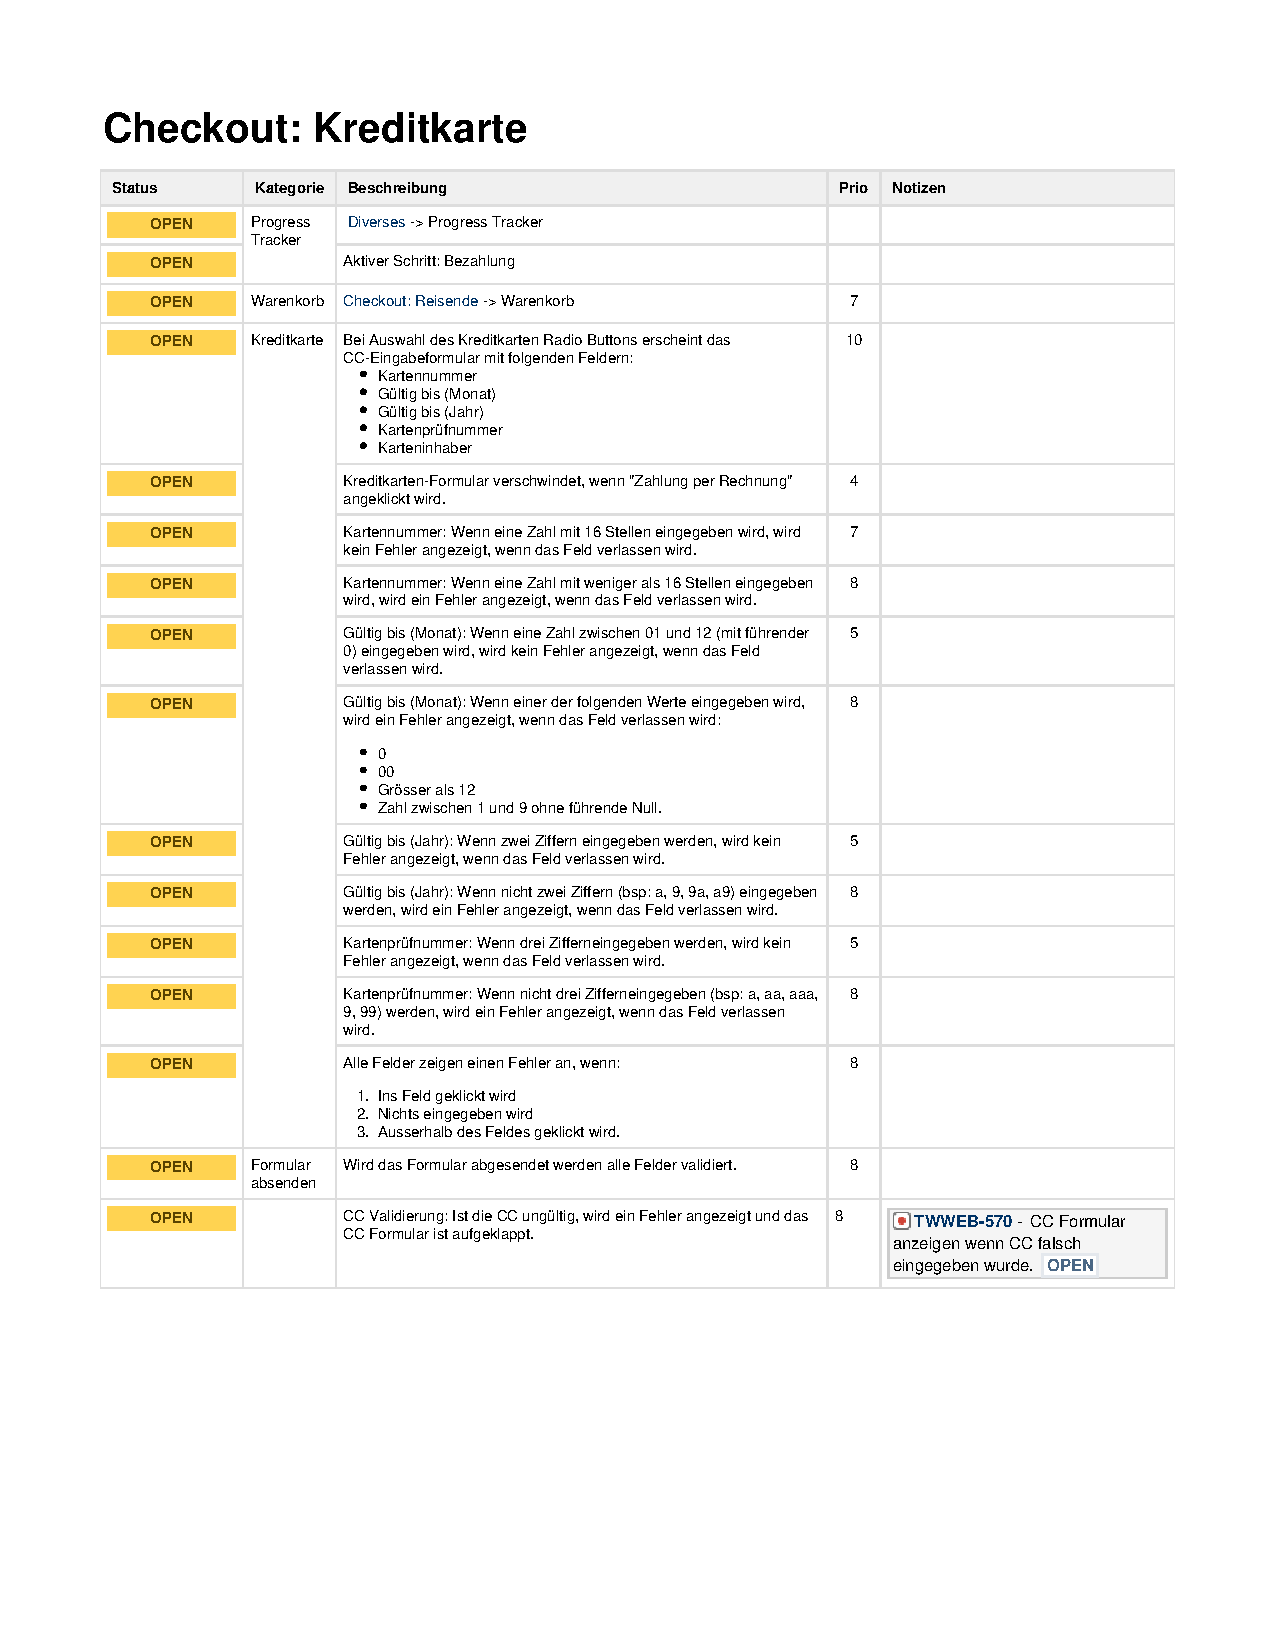
\includepdf[scale=0.8,pages=-,pagecommand=\section{Checkout: Bezahlart}]{./../test-documentation-9-checkout-payment.pdf}


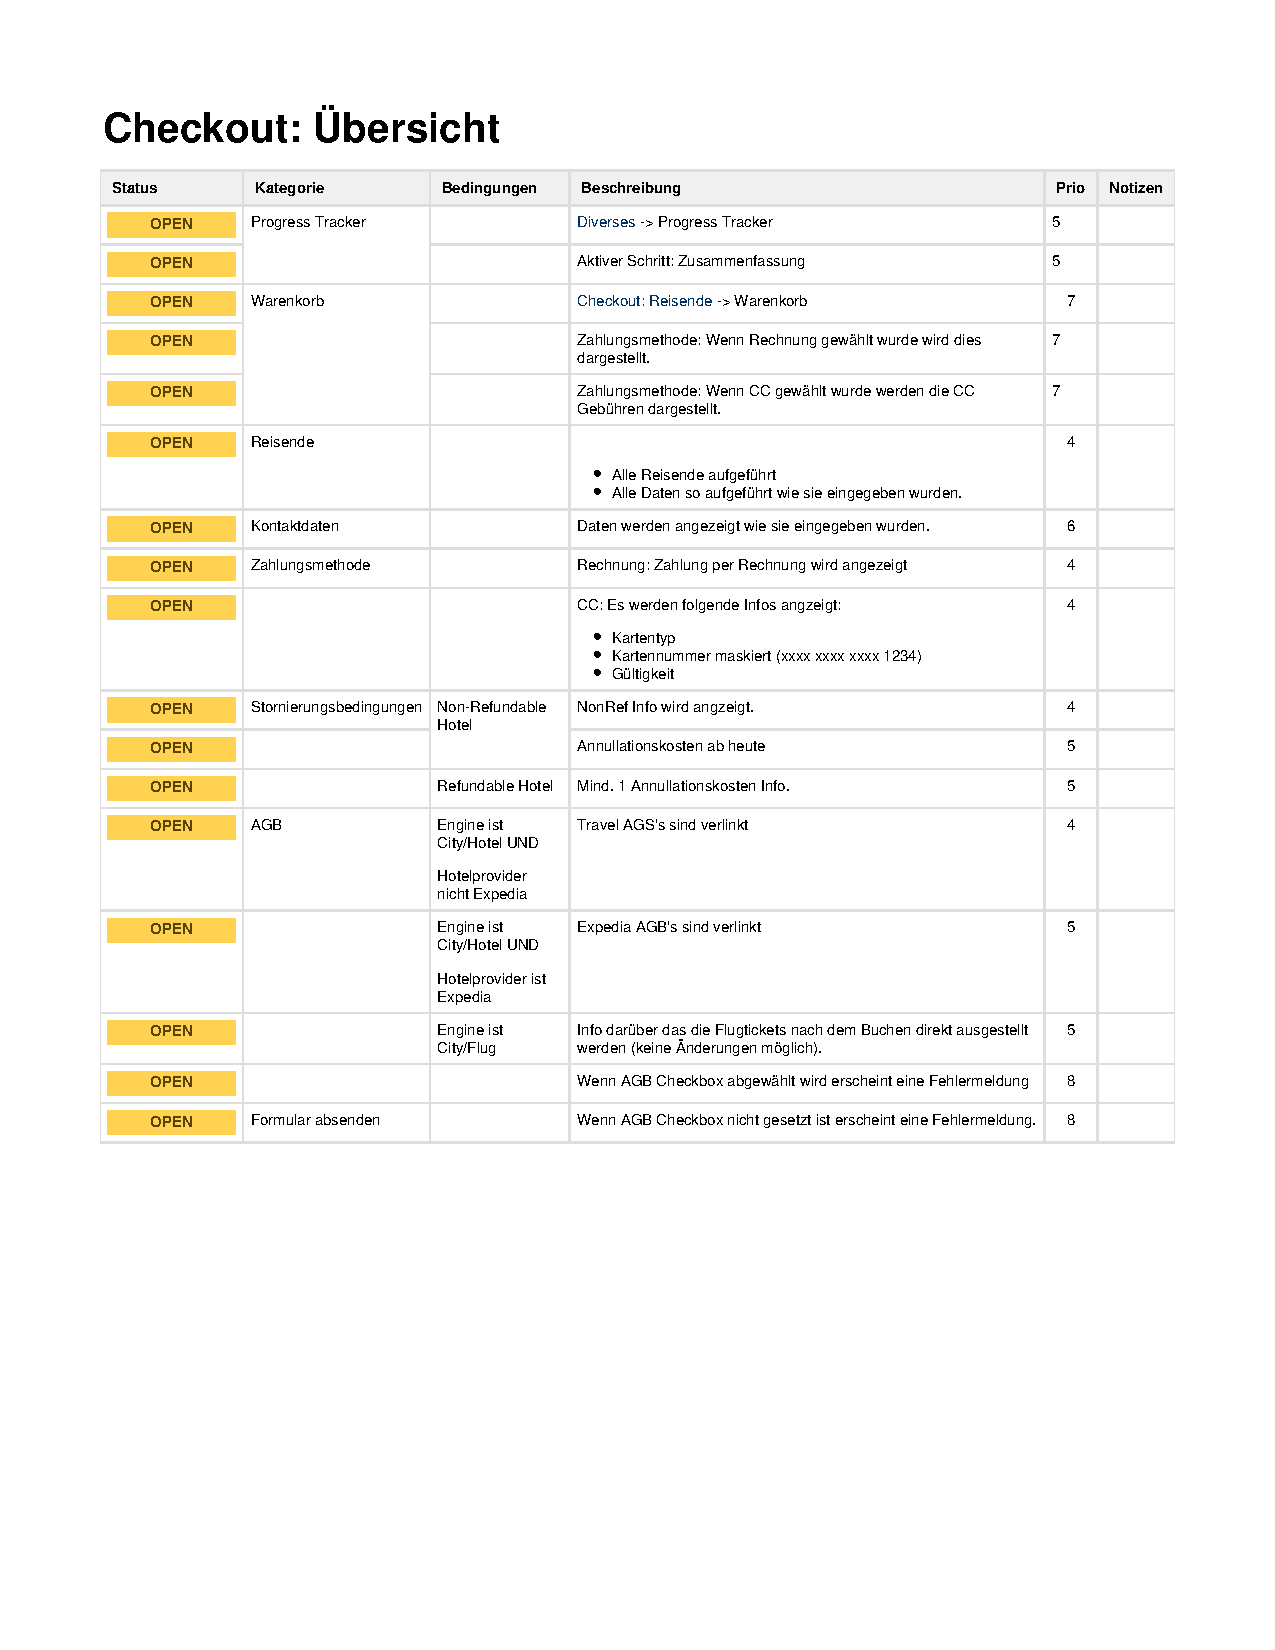
\includepdf[scale=0.8,pages=-,pagecommand=\section{Checkout: Übersicht}]{./../test-documentation-10-checkout-overview.pdf}


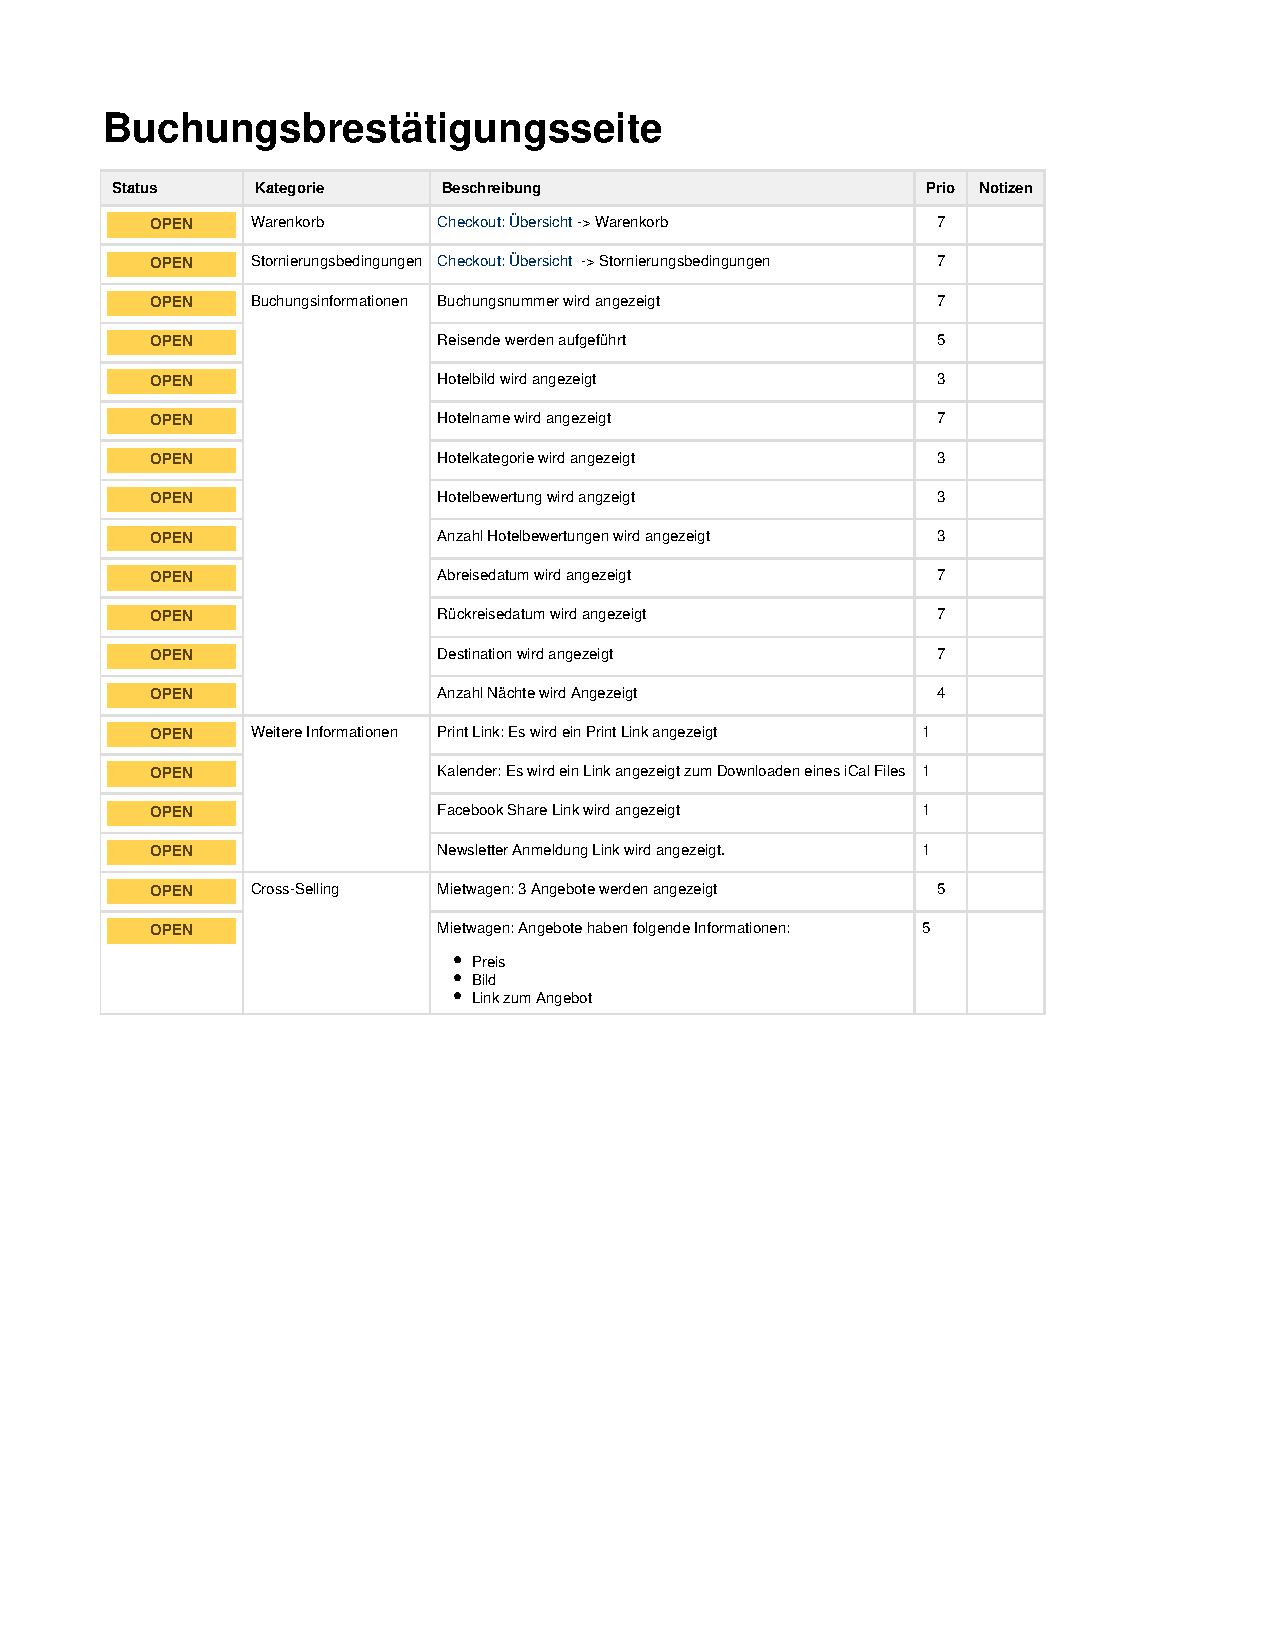
\includepdf[scale=0.8,pages=-,pagecommand=\section{Bestätigungsseite}]{./../test-documentation-11-confirmationpage.pdf}

%\end{document}